\documentclass[a4paper,twoside]{article}

\usepackage{csquotes}
\usepackage[nolist]{acronym}

\usepackage[dvipsnames,table]{xcolor}
\definecolor{darkgreen}{rgb}{0.2, 0.4, 0.33}

\usepackage{booktabs}
\usepackage{multirow}

\usepackage{footnote}
\makesavenoteenv{tabular}
\makesavenoteenv{table}

\usepackage{pifont}%
\newcommand{\yes}{\textcolor{darkgreen}{\ding{51}}} %
\newcommand{\no}{\textcolor{red}{\ding{55}}}%
\newcommand{\questionmark}{\textcolor{darkgray}{\bfseries{\ensuremath{\mathord{?}}}}}
\newcommand{\claimednotreported}{\textcolor{darkgray}{\ding{45}}}

\usepackage{listings}
\usepackage{glossaries}

\usepackage{subcaption}
\usepackage{xfrac}
\usepackage[hidelinks]{hyperref}

\usepackage{epsfig}
\usepackage{subcaption}
\usepackage{calc}
\usepackage{amssymb}
\usepackage{amstext}
\usepackage{amsmath}
\usepackage{amsthm}
\usepackage{multicol}
\usepackage{pslatex}
\usepackage{apalike}

\usepackage{cleveref}

\usepackage{tikz}
\usetikzlibrary{trees,calc,fit,backgrounds,positioning,shapes,snakes,arrows.meta,spy,3d,calendar,shapes.multipart,patterns}

\usepackage{pgfplots}
\usepackage{pgfplotstable}
\usepackage{pgfplotstablefilter}
\pgfplotsset{compat=newest}%
\usepgfplotslibrary{statistics}

\pgfplotsset{
    discard if not/.style 2 args={
        x filter/.code={
            \edef\tempa{\thisrow{#1}}
            \edef\tempb{#2}
            \ifx\tempa\tempb
            \else
                \def\pgfmathresult{inf}
            \fi
        }
    }
}

\pgfplotstableset{
    discard if not/.style 2 args={
        row predicate/.code={
            \def\pgfplotstable@loc@TMPd{\pgfplotstablegetelem{##1}{#1}\of}
            \expandafter\pgfplotstable@loc@TMPd\pgfplotstablename
            \edef\tempa{\pgfplotsretval}
            \edef\tempb{#2}
            \ifx\tempa\tempb
            \else
                \pgfplotstableuserowfalse
            \fi
        }
    }
}

\definecolor{plots-1}{RGB}{228,26,28}
\definecolor{plots-2}{RGB}{55,126,184}
\definecolor{plots-3}{RGB}{77,175,74}
\definecolor{plots-4}{RGB}{152,78,163}
\definecolor{plots-5}{RGB}{255,127,0}
\definecolor{plots-6}{RGB}{153,153,153}
\definecolor{plots-7}{RGB}{166,86,40}

\usepackage{SCITEPRESS}     %

\newcommand{\fixed}{fixed train/test split}
\newcommand{\cvten}{10-fold time-split}
\newcommand{\cveight}{8-fold time-split}
\newcommand{\na}{n/a}

\newcommand{\vocabsize}{\ensuremath{V}}
\newcommand{\topicz}{\ensuremath{z}}
\newcommand{\wordw}{\ensuremath{w}}
\newcommand{\numauthors}{\ensuremath{A}}

\newcommand{\vbq}{\ensuremath{Q}}
\newcommand{\vbp}{\ensuremath{P}}
\DeclareMathOperator*{\argmax}{arg\,max}
\DeclareMathOperator*{\argmin}{arg\,min}

\newcommand{\numtopics}{\ensuremath{K}}
\newcommand{\numiterations}{\ensuremath{R}}
\newcommand{\rndstate}{Random seed}

\newcommand{\ldamodel}{\texttt{LdaModel}}
\newcommand{\ldamulticore}{\texttt{LdaMulticore}}
\newcommand{\atmodel}{\texttt{AuthorTopicModel}}
\newcommand{\paralleltopicmodel}{\texttt{TopicTrainer}}
\newcommand{\vwldacore}{\texttt{lda}}

\newcommand{\gealpha}{\texttt{alpha}}
\newcommand{\geeta}{\texttt{eta}}
\newcommand{\getopics}{\texttt{num\_topics}}
\newcommand{\gerndstate}{\texttt{random\_state}}

\newcommand{\chunksize}{\texttt{chunksize}}
\newcommand{\updateevery}{\texttt{update\_every}}
\newcommand{\decay}{\texttt{decay}}
\newcommand{\offset}{\texttt{offset}}
\newcommand{\gammathreshold}{\texttt{gamma\_threshold}}

\newcommand{\iterations}{\texttt{iterations}}
\newcommand{\passes}{\texttt{passes}}
\newcommand{\workers}{\texttt{workers}}

\newcommand{\vwalpha}{\texttt{--lda\_alpha}}
\newcommand{\vweta}{\texttt{--lda\_rho}}
\newcommand{\vwtopics}{\texttt{--lda}}

\newcommand{\vwchunksize}{\texttt{--minibatch}}
\newcommand{\vwupdateevery}{n/a}
\newcommand{\vwdecay}{\texttt{--power\_t}}
\newcommand{\vwoffset}{\texttt{--initial\_t}}
\newcommand{\vwgammathreshold}{\texttt{--lda\_epsilon}}
\newcommand{\vwrndstate}{\texttt{--random\_seed}}
\newcommand{\vwpasses}{\texttt{--passes}}

\newcommand{\vwiterations}{n/a}

\newcommand{\maalpha}{\texttt{--alpha}}
\newcommand{\maalphaoptimized}{\texttt{--use-symmetric-alpha --alpha}}

\newcommand{\maeta}{\texttt{--beta}}
\newcommand{\matopics}{\texttt{--num-topics}}

\newcommand{\maiterations}{\texttt{--num-iterations}}

\newcommand{\marndstate}{\texttt{--random-seed}}

\newcommand{\maoptinterval}{\texttt{--optimize-interval}}
\newcommand{\maoptburnin}{\texttt{--optimize-burn-in}}
\newcommand{\maworkers}{\texttt{--num-threads}} 

\newcommand{\alphaconcentration}{\ensuremath{\boldsymbol{\alpha_{c}}}}

\newacronym{lda}{LDA}{Latent Dirichlet Allocation}
\newacronym{plsi}{pLSI}{probabilistic Latent Semantic Indexing}
\newacronym{atm}{ATM}{Author-Topic model}
\newacronym{mrr@10}{MRR@10}{Mean Reciprocal Rank @ 10}
\newacronym{mrr@k}{MRR@k}{Mean Reciprocal Rank @ k}
\newacronym{map@10}{MAP@10}{Mean Average Precision @ 10}
\newacronym{map@k}{MAP@k}{Mean Average Precision @ k}
\newacronym{accuracy@k}{Accuracy@k}{Top-k accuracy}
\newacronym{accuracy@10}{Accuracy@10}{Top-10 accuracy}
\newacronym{precision@k}{Precision@k}{Precision@k}
\newacronym{recall@k}{Recall@k}{Recall@k}
\newacronym{f1}{$F_1$}{$F_1$-score}

\newacronym{em}{EM algorithm}{Expectation-Maximization algorithm}

\newacronym{mcmc}{MCMC}{Markov Chain Monte Carlo}
\newacronym{cgs}{CGS}{collapsed Gibbs sampling}
\newacronym{vb}{VB}{Variational Bayes}
\newacronym{bow}{BOW}{Bag-of-Words representation}
\newacronym{svm}{SVM}{Support Vector Machine}
\newacronym{mnb}{MNB}{Multinomial na\"ive Bayes classifier}

\newacronym{cosine}{\ensuremath{D_{\scriptscriptstyle\text{Cos}}}}{Cosine distance}
\newacronym{manhattan}{\ensuremath{D_{\scriptscriptstyle\text{Man}}}}{Manhattan distance}
\newacronym{js}{\ensuremath{D_{\scriptscriptstyle\text{JS}}}}{Jensen-Shannon distance}
\newacronym{jaccard}{\ensuremath{D_{\scriptscriptstyle\text{Jac}}}}{Jaccard distance}

\newcommand{\mallet}{\textit{MALLET}}
\newcommand{\gensim}{\textit{Gensim}}
\newcommand{\vw}{\textit{Vowpal Wabbit}}
\newcommand{\tomotopy}{\textit{tomotopy}}
\newcommand{\gibbslda}{\textit{GibbsLDA++}}
\newcommand{\jgibblda}{\textit{JGibbLDA}}
\newcommand{\stmt}{\textit{Stanford Topic Modeling Toolbox}}
\newcommand{\mtmt}{\textit{Matlab Topic Modeling Toolbox}}
\newcommand{\stmtshort}{\textit{Stanford TMT}}
\newcommand{\mtmtshort}{\textit{Matlab TMT}}
\newcommand{\sklearn}{\textit{scikit-learn}}

\newcommand{\nltk}{\textit{NLTK}}

\newcommand{\vargserver}{\textit{VARG-server}}

\newcommand{\cpp}{C\nolinebreak[4]\hspace{-.05em}\raisebox{.4ex}{\tiny\bfseries ++}}
\newcommand{\clang}{C}

\newcommand*\mean[1]{\overline{\text{#1}}}

\newcommand{\mozff}{Mozilla Firefox}
\newcommand{\mozcore}{Mozilla Core}
\newcommand{\chromium}{Chromium}
\newcommand{\basemeasure}{\ensuremath{m}}

\newglossaryentry{latex}
{
    name=latex,
    description={Is a mark up language specially suited for scientific documents}
}
\newglossaryentry{alpha}
{
    name=\ensuremath{\alpha},
    description={Hyperparameter that defines a Dirichlet distribution used as a prior for the topic distributions $\theta$}
}
\newglossaryentry{beta}
{
    name=\ensuremath{\beta},
    description={Hyperparameter that defines a Dirichlet distribution used as a prior for the topic-term distributions $\phi$}
}
\newglossaryentry{phi}
{
    name=\ensuremath{\phi},
    description={Posterior distribution of the topics, also known as topic-term distributions}
}
\newglossaryentry{theta}
{
    name=\ensuremath{\theta},
    description={Posterior distribution of the topic proportions, also known as document-topic distributions for LDA or author-topic distributions for ATM}
}

\newglossaryentry{numtopics}
{
    name=\ensuremath{K},
    description={Hyperparameter that specifies the number of topics learned from the data}
}
\newglossaryentry{vocabulary}
{
    name=\ensuremath{V},
    description={Each observed word is an instance of an element in a fixed vocabulary of \ensuremath{V} terms}
}

\newglossaryentry{numprocessors}
{
    name=\ensuremath{P},
    description={Degree of parallelism used for training of \glsentryname{lda} models, i.e., the number of threads or processes run in parallel}
}

\newglossaryentry{minibatch}
{
    name=\ensuremath{S},
    description={Hyperparameter that specifies the batch size used in online Variational Bayes LDA}
}

\newglossaryentry{kappa}
{
    name=\ensuremath{\kappa},
    description={Learning rate used in online Variational Bayes LDA}
}

\newglossaryentry{tau}
{
    name=\ensuremath{\tau_0},
    description={Learning parameter that downweights early iterations in online Variational Bayes LDA}
}
\newglossaryentry{meanchangethreshold}
{
    name=\ensuremath{\delta},
    description={Threshold value used in Variational Bayes inference to determine convergence}
}

\newglossaryentry{numiterationsgibbs}
{
    name=\ensuremath{i_{\scriptscriptstyle\text{CGS}}},
    description={Hyperparameter that specifies the number of iterations run for \glsentryname{cgs}-based LDA implementations}
}

\newglossaryentry{numiterationsvb}
{
    name=\ensuremath{i_{\scriptscriptstyle\text{VB}}},
    description={Hyperparameter that specifies the maximum number of iterations for updating the document-topic distributions in the E-step for \glsentryname{vb}-based LDA implementations}
}

\newglossaryentry{dretom-tradeoff}
{
    name=\ensuremath{\vartheta},
    description={Hyperparameter for developer recommendation to balance developers expertise and interest}
}

\newglossaryentry{vblong}
{
    name={Variational Bayes},
    description={Technique used for inference of the posterior probability in probabilistic topic models}
}

\newglossaryentry{gibbs}
{
    name={Gibbs sampling},
    description={Technique used for inference of the posterior probability in probabilistic topic models}
}

\newglossaryentry{topkaccuracy}
{
    name={Top-k accuracy},
    description={Evaluation metric that computes the number of times where the correct label is among the top k labels predicted (ranked by predicted scores)}
}

\newglossaryentry{top10accuracy}
{
    name={Top-10 accuracy},
    description={Top-k accuracy with k = 10, also known as rank-10 accuracy, HitRate@10 or Accuracy@10}
}
\newglossaryentry{mrr}
{
    name={Mean Reciprocal Rank @ k},
    description={Evaluation metric that considers the rank of the correct label among the top k labels predicted (ranked by predicted scores)}
}
\newglossaryentry{map}
{
    name={Mean Average Precision @ k},
    description={Evaluation metric that considers the rank of multiple correct labels among the top k labels predicted}
}

\newglossaryentry{dretom}
{
    name={DRETOM},
    description={Baseline approach for developer recommendation on bug reports using LDA by~\cite{xie2012dretom}}
}

\newglossaryentry{dratom-theta}
{
    name={DRATOM(\ensuremath{\vartheta})},
    description={Our proposed method builds on DRETOM but uses the Author-Topic model instead of Latent Dirichlet Allocation}
}

\newglossaryentry{dratom}
{
    name={DRATOM},
    description={Our proposed method advances \glsentryname{dratom-theta} by better utilizing the Author-Topic model, removing the burden of specifying \glsentryname{dretom-tradeoff} in advance}
}

\newglossaryentry{drasim}
{
    name={DRASIM},
    description={Our proposed method utilizes the Author-Topic model to measure similarity between developers and issue reports in a joint topic space}
}

\newglossaryentry{onlineldavb}
{
    name={online VB LDA},
    description={Online Variational Bayes algorithm for Latent Dirichlet Allocation by~\cite{Hoffman2010OnlineLDA}}
}

\newglossaryentry{batchldavb}
{
    name={batch VB LDA},
    description={Batch Variational Bayes algorithm for Latent Dirichlet Allocation by~\cite{Blei2003LatentAllocation}}
}

\newglossaryentry{emalgo}
{
    name={Expectation-Maximization algorithm},
    description={Iterative method to find (local) maximum likelihood estimates of latent variables}
}

\newglossaryentry{estep}
{
    name={E-step},
    description={Expectation step of EM algorithm which creates a function for the expectation of the log-likelihood evaluated using the current estimate for the parameters}
}

\newglossaryentry{mstep}
{
    name={M-step},
    description={Maximization step of EM algorithm which computes parameters maximizing the expected log-likelihood found on the E-step}
}

\usepackage{xspace}
\makeatletter
\DeclareRobustCommand\onedot{\futurelet\@let@token\@onedot}
\def\@onedot{\ifx\@let@token.\else.\null\fi\xspace}
\def\etal{et~al\onedot}
\def\eg{e.g\onedot,\xspace} 
\def\ie{i.e\onedot,\xspace} 
\def\etc{etc\onedot} 
\def\vs{vs\onedot}
\makeatother

\begin{acronym}
\acro{AST}{Abstract Syntax Tree}
\acro{ATM}{Author-Topic Model}
\acro{DTM}{Developer-Topic Model}
\acro{LDA}{Latent Dirichlet Allocation}
\acro{LSI}{Latent Semantic Indexing}
\acro{LOC}{Lines-of-Code}
\acro{NLP}{Natural Language Processing}
\acro{MBTI}{Myers-Briggs Type Indicator}
\acro{MDS}{Multidimensional Scaling}
\acro{MTM}{Multi-feature Topic Model}
\acro{SE}{Software Engineering}
\acro{BOW}{Bag-of-Words}
\acro{TTM}{Tag-Topic Model}
\acro{VCS}{Version Control System}
\acro{kNN}{k-Nearest-Neighbors}
\acro{NN}{Nearest Neighbor}
\acro{MRR}{Mean Reciprocal Rank}
\acro{DRETOM}{Developer Recommendation based on Topic Models}
\acro{DRATOM}{Developer Recommendation based on the Author-Topic Model}
\acro{DRATOMBayes}{Developer Recommendation based on the Author-Topic Model and Bayes Formula}
\acro{DRASIM}{Developer Recommendation based on Author Similarity}
\acro{CGS}{Collapsed Gibbs Sampling}
\acro{VB}{Variational Bayes}
\acro{OVB}{Online Variational Bayes}
\acro{SVM}{Suport Vector Machine}
\acro{KL}{Kullback Leilber divergence}
\acro{OSS}{Open Source Software}
\acro{MRR}{Mean Reciprocal Rank}
\acro{MAP}{Mean Average Precision}
\end{acronym}

\begin{document}

\title{Mining Developer Expertise from Bug Tracking Systems using~the~Author-Topic~Model}

\author{
\authorname{
    Daniel Atzberger\footnotemark[1],
    Jonathan Schneider\thanks{Both authors contributed equally to this work.},
    Willy Scheibel\orcidAuthor{0000-0002-7885-9857},\\
    Daniel Limberger\orcidAuthor{0000-0002-9111-4809},
    Matthias Trapp\orcidAuthor{0000-0003-3861-5759},
    and Jürgen Döllner}
    \affiliation{Hasso Plattner Institute, Digital Engineering Faculty, University of Potsdam, Germany}
}

\keywords{Bug Triaging, Topic Models, Latent Dirichlet Allocation, Author-Topic Model}

\inofficialcopyrightnotice{Author's Version. This paper is originally published in the Proceedings of the 17th International Conference on Evaluation of Novel Approaches to Software Engineering -- ENASE, 107--118, 2022, and is accessible on \textsc{SciTePress}: \url{https://doi.org/10.5220/0011045100003176}}

\abstract{
During the software development process, software defects, so-called bugs, are captured in a semi-structured manner in a bug tracking system using textual components and categorical features.
It is the task of the triage owner to assign open bugs to developers with the required skills and expertise. 
This task, known as \textsl{bug triaging}, requires in-depth knowledge about a developer's skills.
Various machine learning techniques have been proposed to automate this task, most of these approaches apply topic models, especially Latent Dirichlet Allocation, for mining the textual components of bug reports.
However, none of the proposed approaches explicitly models a developer's expertise.
In most cases, these algorithms are treated as a black box, as they allow no explanation about their recommendation.
In this work, we show how the Author-Topic Model, a variant of Latent Dirichlet Allocation, can be used to capture a developer's expertise in the latent topics of a corpus of bug reports from the model itself.
Furthermore, we present three novel bug triaging techniques based on the Author-Topic Model.
We compare our approach against a baseline model, that is based on Latent Dirichlet Allocation, on a dataset of 18\thinspace{}269 bug reports from the Mozilla Firefox project collected between July 1999 to June 2016.
The results show that the Author-Topic Model can outperform the baseline approach in terms of the Mean Reciprocal Rank.
}

\onecolumn
\maketitle \normalsize \setcounter{footnote}{0} \vfill

\section{\uppercase{Introduction}}
\label{sec:introduction}
Today's software projects are characterized by a large number of developers involved and an ever increasing structural and behavioral complexity.
This is the main cause for the emergence of software misbehavior, called bugs. 
When a bug is detected, it is described by a bug report within an issue tracking or bug tracking system in a semi-structured manner.
Besides textual components, \eg a title and a more detailed description, bug reports use categorical attributes, \eg the product, the affected component, the version, and the priority and severity, to specify details.
Additionally, files can be attached and solutions can be discussed.
Based on this rich source of information, it is the task of the bug triage owner to assign the bug report to a developer to fix it.
This process is known as bug triaging.
In order to ensure high productivity, it is necessary that the developer to solve the bug has the required skills and expertise~\cite{sommerville2016softwareengineering}.
In most cases, the decisions made by the triage owner are based on subjective perceptions~\cite{Zou2020HowTechniques}, that in turn often lead to wrong assignments, which might result in a delay in the development process.

Automated bug triaging techniques try to overcome this issue by mining the information contained in a bug tracking system~\cite{Sajedi-Badashian2020GuidelinesResearch,Zou2020HowTechniques,Zhang2015AAnalysis}.
Most of these approaches analyze closed bug reports with known bug resolvers to train a machine learning algorithm that can then in turn be used to rank developers for a new bug.
A large class of those techniques models the textual components of bug reports using a probabilistic topic model, mostly \ac{LDA}~\cite{blei2003latent}.
The goal of \ac{LDA} is to extract semantic clusters in the vocabulary, given as distributions over this vocabulary, by examining patterns of co-occurring words within bug reports.
The semantic structure of bug reports can then in turn be described as multinomial distributions over the topics.
The results of the \ac{LDA} model are then used as input for the machine learning model.
Though it has shown great advances in the last years, \ac{LDA} is not able to describe a developer's expertise directly from the available data.
As such, these models provide no explanation to the user, which is a limiting factor for their applicability in a real-world setting~\cite{Aktas2020AutomatedCase,Zou2020HowTechniques}.

In this work, we apply the \ac{ATM} on a corpus of closed bug reports with known resolvers, to model a developer's expertise in the latent topics~\cite{rosen-zvi2004authors}.
Based on this description of a developer, we modify an existing bug triaging algorithm, named \ac{DRETOM}, based on \ac{LDA}, proposed by Xie \etal (2012).
This results in three alternative methods for automated bug triaging, namely
\begin{enumerate}
    \item \ac{DRATOM},
    \item \ac{DRATOMBayes}: a further iteration of \ac{DRATOM}, which makes use of the Bayes formula for conditional probabilities,
    \item \ac{DRASIM}: By applying the \ac{ATM} on past bug reports, developers and bug reports can be described in a joint feature space. This reduces the bug triaging task to a \ac{NN} search.
\end{enumerate}
We further evaluate the effectiveness of the \ac{ATM} and the influence of its hyperparameters for the bug triaging task.
For this purpose, we use a publicly available dataset of 18\thinspace{}269 bug reports from the Mozilla Firefox project, collected between July 1999 and June 2016.
The results show that our modification of \ac{DRETOM} is able to outperform the baseline approach in terms of the \ac{MRR}.

The remainder of this work is structured as follows:
Section \ref{section: related work} presents existing approaches for bug triaging, which apply \ac{LDA} for modeling the textual components of bug reports. 
In Section \ref{section: lda} we give a short overview of \ac{LDA} and its variant \ac{ATM}.
We detail our three novel bug triaging algorithms, based on the \ac{ATM}, in section \ref{section: atm}.
We describe the experimental setup in section \ref{section: experiment} and discuss its results in section \ref{section: results}.
Section \ref{section: conclusion} concludes this paper and outlines directions for future work.

\section{\uppercase{Related Work}}
\label{section: related work}

Various machine learning and information retrieval approaches for bug triaging have been proposed~\cite{Sajedi-Badashian2020GuidelinesResearch}.
We focus our presentation of the related work on approaches that apply probabilistic topic models on the textual components of bug reports.
We therefore disregard work that utilizes data from version control systems~\cite{Matter2009AssigningDevelopers,Kagdi2012AssigningDevelopers,Shokripour2013WhyRecommendation,Khatun2016ADevelopers,Hu2014EffectiveInformation} or question-and-answer platforms~\cite{Sajedi-Badashian2015CrowdsourcedTriaging}. %
Here, we want to clarify that we always refer to bug reports, even though issue reports or change requests are also common terms used in the literature.
Precisely, we refer to the problem defined as follows:
\enquote{Given a new bug report, identify a ranked list of developers whose expertise qualifies them to fix the bug}~\cite{Sajedi-Badashian2020GuidelinesResearch}.

Xie \etal were the first to apply \ac{LDA} for the bug triaging task~\cite{xie2012dretom}.
Their approach \ac{DRETOM} models a developer's interest and expertise in topics from a corpus of historical bugs for recommending suitable contributors for an open bug.
As our approach builds upon the work of Xie \etal, we will present a detailed description of it in \Cref{section: atm}.

Based on the work of Xie \etal (2012), successive work focused on improving the quality of developer recommendations considering additional input features of a bug report~\cite{xia2013accurate,naguib2013bug,zhang2014novel,yang2014towards,nguyen2014topic,zhang2016towards,xia2016improving,zhang2014butter}.
What all approaches have in common is that for each bug report, the title and description are used to determine the latent topics.

Given a bug report, Xia \etal extract a feature vector that captures the topics via \ac{LDA}, the affected product, and components of the bug report~\cite{xia2013accurate}.
Using a newly defined distance metric, the algorithm recommends a set of developers who are assigned to a new bug report.

Naguib \etal proposed an approach leveraging \ac{LDA} and the developer activities, such as reviewing, fixing, and assigning bug reports~\cite{naguib2013bug}.
First, they use in addition to a bug report's title and description its system component to categorize bug reports into topics.
Subsequently, they create an activity profile for each developer, so that it can be used alongside the topic associations to recommend a suitable developer.

Zhang \etal also utilized \ac{LDA} to extract topics from historical bug reports~\cite{zhang2014novel}.
In addition, they analyzed the relationship between the developers, \ie assignees, commenters, and the bug reporter whose bug reports attracted the most number of comments.

Yang \etal proposed a new method by utilizing not only the natural language for \ac{LDA}, but multiple features including product, component, severity, and priority~\cite{yang2014towards}.
They extract the set of candidate developers who have contributed to the bug reports having the same combination of topic and features and rank them by the scores determined using their number of activities, \ie a developer's number of commits, comments, attachments, and bug assignments.

Zhang \etal use structural information from the submitter-bug-commenter heterogeneous network to improve the quality of developer recommendations~\cite{zhang2014butter}.
Through this network, submitters and commenters obtain the topic information propagated from bugs, which adjust the topic distributions obtained by the \ac{LDA} model.

Nguyen \etal used the inferred topics from \ac{LDA} along with the bug fixer and the severity levels of historical bug reports as an input of a log-normal regression model for predicting defect resolution time~\cite{nguyen2014topic}.
Based on each developer's mean time to repair and dependent on the most prominent topic of the open bug report, they recommend the developer that is likely the fastest in resolving the issue.

In a later work, Zhang \etal proposed a new similarity measure to find related historical bug reports based on its title, description, product, and component~\cite{zhang2016towards}.
Their approach uses 18 hyperparameters that need to be tuned to weight the individual features, of which only the number of topics is a hyperparameter of the underlying \ac{LDA} model.
The other hyperparameters of \ac{LDA} remain on the default settings of the respective \ac{LDA} implementation.
For the actual developer recommendation, that also incorporates a developer's number of comments, fixed and reopened bugs, there are two more hyperparameters to be tuned.

Xia \etal proposed the \ac{MTM}, a method that extends the basic topic modeling algorithm \ac{LDA}~\cite{xia2016improving}.
The \ac{MTM} includes a bug report's feature combination, \eg its product and component, as an additionally observed variable, and models the topic distributions for each feature combination.
Their approach recommends the developers based on the affinity score towards a topic and the feature combination.

A detailed overview on how topic models are used for software engineering tasks in general is presented by Chen \etal (2016).~\nocite{chen2016survey}

\section{Latent Dirichlet Allocation}
\label{section: lda}

\begin{figure*}[t]
    \subcaptionbox{\label{fig:dirichlet-uniform}$\alpha = (1,1,1)$ with $a_c=3$}
    {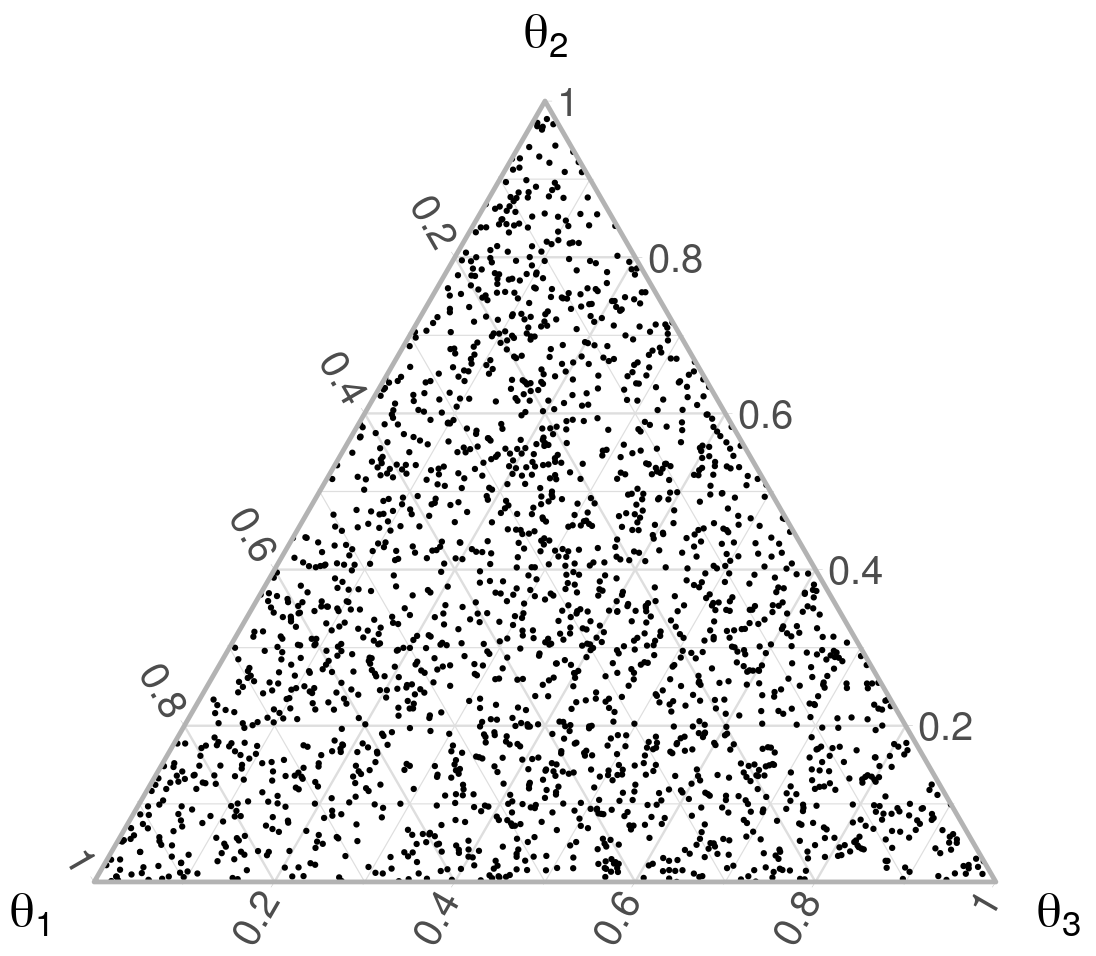
\includegraphics[width=0.32\textwidth]{figures/Dirichlet/Dirichlet_uniform}}%
    \hfill%
    \subcaptionbox{\label{fig:dirichlet-concentrated}$\alpha = (10,10,10)$ with $a_c=30$}
    {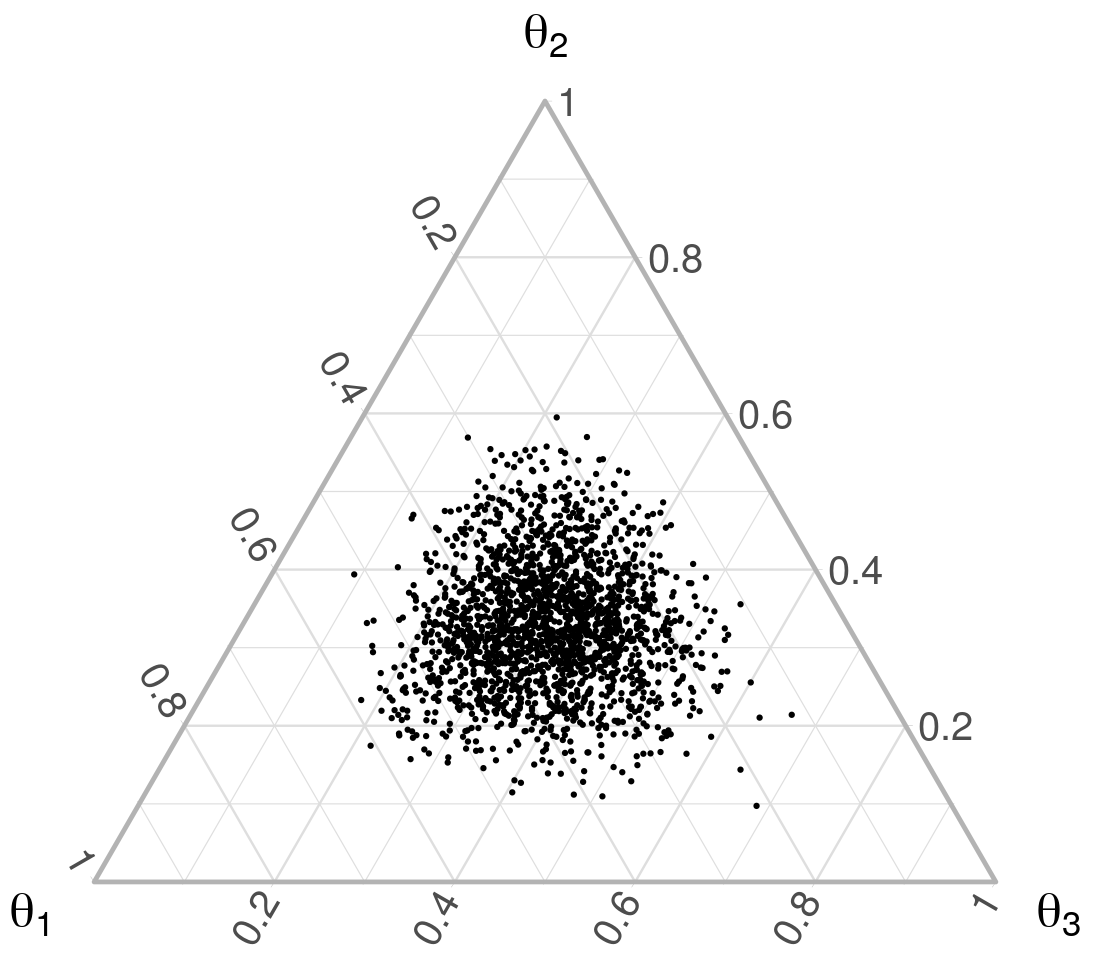
\includegraphics[width=0.32\textwidth]{figures/Dirichlet/Dirichlet_concentrated}}%
    \hfill%
    \subcaptionbox{\label{fig:dirichlet-spreadout}$\alpha = (0.1,0.1,0.1)$ with $a_c=0.3$}
    {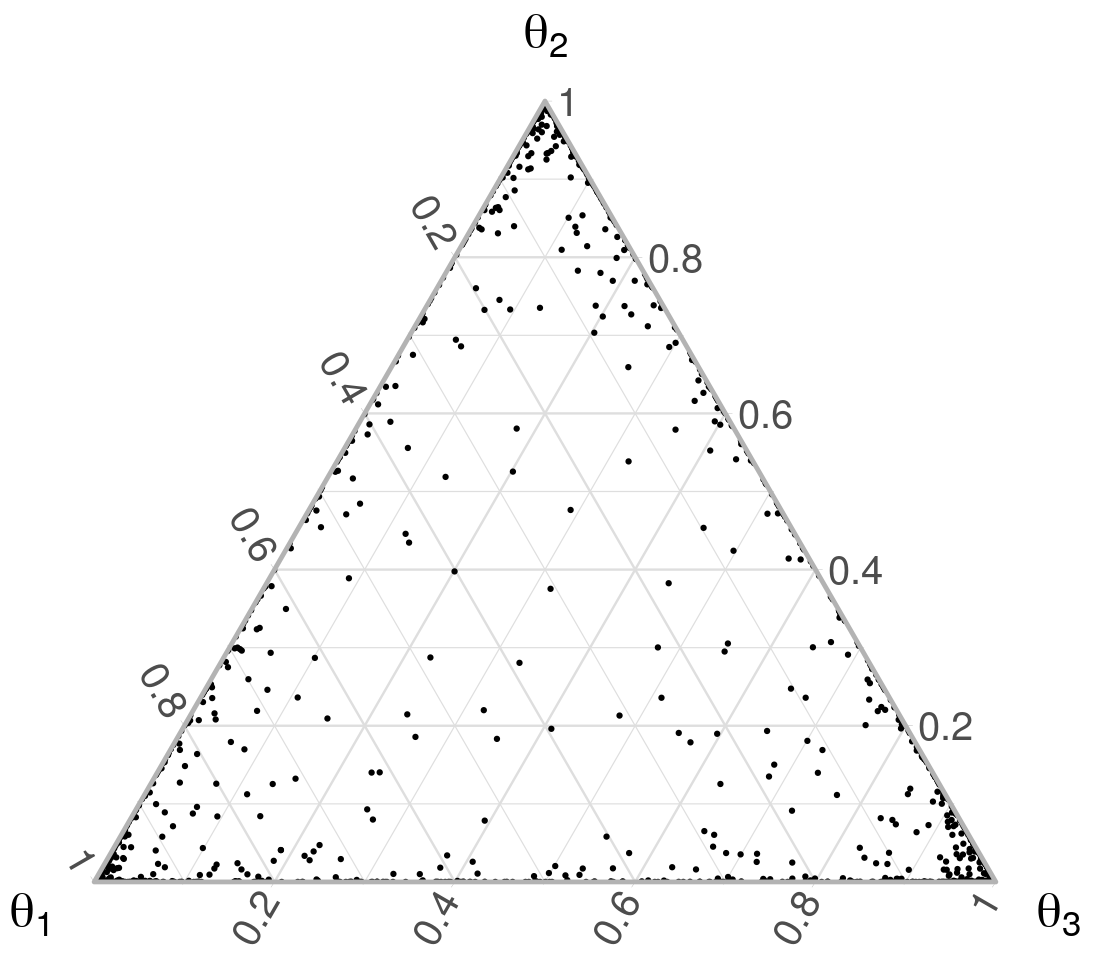
\includegraphics[width=0.32\textwidth]{figures/Dirichlet/Dirichlet_spreadout}}%
    \caption[Impact of concentration parameter $a_c$ on symmetrical Dirichlet distributions]
    {2,000 randomly sampled topic distributions $\theta$ using varying concentration parameters $a_c$ for symmetrical Dirichlet prior $\alpha$.
    We illustrate the distributions for $K=3$ topics in the three-dimensional topic space $\theta=(\theta_1,\theta_2,\theta_3)$.
    The base measure $\basemeasure{}=\left(\sfrac{1}{3},\sfrac{1}{3},\sfrac{1}{3}\right)$ is uniform for every symmetrical Dirichlet distribution.
    }
    \label{fig:dirichlet-alpha-priors}
\end{figure*}

In this section we give a short overview on \ac{LDA} required to understand the rest of our work.
Topic models are a widely used technique for mining the semantic structure of a collection of documents, \eg for summarization or classification tasks~\cite{aggarwal2012mining}.
The by far most popular topic model for mining software repositories is \ac{LDA} proposed by Blei \etal~\cite{chen2016survey,Sun2016ExploringSurvey}.
Given a corpus $\mathcal{C} = \{d_1, \dots, d_m\}$, where each element $d_1, \dots, d_m$ denotes a single document stored as a \ac{BOW}, \ac{LDA} extracts latent topics $\varphi_1, \dots, \varphi_K$, where the number of topics $K$ is a hyperparameter of the model~\cite{blei2003latent}.
The topics $\varphi_1, \dots, \varphi_K$ are given as multinomial distributions over the vocabulary $\mathcal{V}$ of the corpus $\mathcal{C}$.
In most cases the most probable words are a strong indicator for the \enquote{concept} underlying a topic.
\Cref{tab:topics_ff} shows an example for three topics with their ten most probable words that were extracted from the Mozilla Firefox corpus, which we will describe in detail in \Cref{ssec: dataset}.
\ac{LDA} further results in descriptions $\theta_1, \dots, \theta_m$ of the documents $d_1, \dots, d_m$ as multinomial distributions over the set of topics.
The vectors $\theta_1, \dots, \theta_m$ therefore capture the semantic structure of the documents and allow a formal comparison using a dissimilarity measure, \eg the cosine-similarity or the Jensen-Shannon distance.
The generative process underlying \ac{LDA} is given by

\begin{table}[t]
    \footnotesize
    \centering
	\setlength{\tabcolsep}{15.0pt}%
	\renewcommand{\arraystretch}{1.0}
    \caption[The three extracted topics with the highest probability from the exemplary bug report]
    {Three extracted topics from \mozff{}.
    For each topic, the ten most probable terms are displayed.
    }
    \begin{tabular}{c|c|c}
    \toprule
    \textbf{Topic \#1} & \textbf{Topic \#2} & \textbf{Topic \#3} \\ \midrule
     private & preferences &          bar \\
    browsing &        pref &          url \\
        mode &     options &     location \\
       clear &      dialog & autocomplete \\
     cookies &     default &         text \\
     history &         set &      address \\
      window &       prefs &      results \\
        data &      option &         type \\
      cookie &  preference &        enter \\
       cache &      change &       result \\\hline

    \end{tabular}
    \label{tab:topics_ff}
\end{table}


\begin{enumerate}
    \item For each document $d$ in the corpus $\mathcal{D}$ choose a distribution over topics $\theta \sim \text{Dirichlet}(\alpha)$
    \item For each word $w$ in $d$
    \begin{enumerate}
        \item Choose a topic $z \sim \text{Multinomial}(\theta)$
        \item Choose the word $w$ according to the probability $p(w \vert z, \beta)$
    \end{enumerate}
\end{enumerate}

The hyperparameter $\alpha = (\alpha_1, \dots, \alpha_K)$, where $0 < \alpha_i$ for all $1\le i \le K$, is called the Dirichlet prior for the document-topic distribution.
It is often written as the product $\alpha = a_c \cdot m$ of its concentration parameter $a_c \in \mathbb{R}$ and its base measure $m = (m_1, \dots, m_K)$, which is a vector whose components sum up to one.
In the case of $m_1 = \dots = m_K = \sfrac{1}{K}$, the Dirichlet prior $\alpha$ is said to be symmetric.
\Cref{fig:dirichlet-alpha-priors} illustrates the effect of the chosen Dirichlet prior $\alpha$.

The parameter $\beta = (\beta_1, \dots, \beta_N)$, where $0 < \beta_i$ for $1\le i \le N$ and $N$ denotes the size of the vocabulary $\mathcal{V}$, \ie the set of words in the corpus $\mathcal{C}$, is the Dirichlet prior for the topic-term distribution.

As inference for \ac{LDA} is intractable, it is required to apply approximation techniques~\cite{blei2003latent}.
Popular examples include Collapsed Gibbs Sampling (CGS)~\cite{Griffiths2004FindingTopics}, Variational Bayes (VB)~\cite{blei2003latent}, and its online version (OVB)~\cite{Hoffman2010OnlineLDA}.

Many variants of \ac{LDA} have been developed taking into account additional meta information about the documents of a corpus, \eg Labeled LDA which makes use of tags attached to the documents, thus resulting in topics with a defined label~\cite{ramage2009labeled}.
The \ac{ATM} is another such variant, which takes information about authorship into account.
The \ac{ATM} is based on a generative process, similar to that of \ac{LDA}, which assumes that each document is written in a collaborative manner by its authors, who are observed as additional information~\cite{rosen-zvi2004authors}.
In addition to the document-topic distributions, the \ac{ATM} learns representations of the authors as distributions over the topics.
\ac{LDA} can be seen as a special case of the \ac{ATM}, where each file has one unique author.
To the best of our knowledge, the \ac{ATM} was only used for a software engineering task in the work of Linstead \etal for mining developer activities on the Eclipse source code~\cite{linstead2007eclipseeeveloper,Linstead2009Sourcerer:Repositories}.
When applied to historical bug reports, each developer who has contributed to bug fixing can be described as a distribution over topics.

\section{Mining Bug Reports with Author-Topic-Models}
\label{section: atm}

The approach \ac{DRETOM} follows three steps.
First, an \ac{LDA} model is trained on a corpus of historical bug reports, then associations between developers and topics are constructed using a heuristic, and finally authors are recommended for incoming bug reports according to some ranking scheme.
In this section, we present three approaches to how the \ac{ATM} can be utilized for the bug triaging task by taking its capability to relate developers and topics into account.
It has to be noted that in the context of bug triaging, we denote the resolver of the bug report as the author, who should not be confused with the reporter of a bug.
As our first two approaches are modifications of \ac{DRETOM}, we start with a description of the approach by Xie \etal (2012).~\nocite{xie2012dretom}
Our first approach (\ac{DRATOM}) is derived from \ac{DRETOM} by simply replacing its \ac{LDA} core with the \ac{ATM}.
The second modification (\ac{DRATOMBayes}) utilizes the relation between developers and topics learned from the \ac{ATM}, thus making the heuristic and trade-off parameter $\theta$ from \ac{DRETOM} redundant.
Our third approach makes full use of the \ac{ATM} by modeling developers as well as bug reports in a joint feature space, thus reducing the bug triaging task to a \ac{NN} search.

\subsection{Preprocessing}
\label{ssec: preprocessing}
In the remainder of this work, we view each bug report as a document consisting of its title and a more detailed description.
Discussions below the bug report are not taken into account, as they are not available during the entire lifecycle of a bug, especially not during the first assignment.
When applying topic models, it is common to undertake several preprocessing steps, in order to remove noise in the vocabulary~\cite{chen2016survey}.
It further reduces the size of the vocabulary thus accelerating the computation time.
Our preprocessing pipeline follows the best-practice recommendations systematically studied by Schofield \etal~\cite{Schofield2017UnderstandingAllocation,Schofield2017PullingModels,Schofield2017QuantifyingModels}:
\begin{enumerate}
    \item Removal of URL, hex code, stack trace information, timestamps, line numbers, tokens starting with numerics, tokens consisting of only one character and punctuation,
    \item Lower casing the entire document,
    \item Removal of all words from the English \textit{NLTK Stopwords Corpus}\footnote{\url{http://www.nltk.org/nltk\_data/}}
    \item We remove words with a frequency less than 5, we further remove words that occur in more than 20\% across all bug reports.
\end{enumerate}
In particular, in contrast to Xie \etal (2012) we do not apply stemming, as words with the same morphological roots are often placed in the same topic, thus making stemming redundant and might damage models~\cite{Schofield2016ComparingModels}.
After preprocessing, all bug reports are stored as \ac{BOW}.

\subsection{DRETOM}
In the first step of \ac{DRETOM}, an \ac{LDA} model is trained on a corpus of historical bug reports and each of these bug reports is assigned to the topic of its maximum probability.
Additionally, all collaborators for the historical bug reports are extracted from the bug tracking system.

The suitability of a developer d to solve a bug b is given by the conditional probability $P(\text{d} \vert \text{b})$.
This probability can be computed as the sum
\begin{align}
    P(\text{d} \vert \text{b}) = \sum \limits_{\text{z}} P(\text{d} \vert \text{z}) \cdot P(\text{z} \vert \text{b}), \label{eq:DRETOM}
\end{align}
where $P(\text{d} \vert \text{z})$ denotes the skill level of the developer d in the respective topic z, and $P(\text{z} \vert \text{b})$ is the probability of the topic in the given bug report.
The skill of developer d in topic z comprises two parts, his interest $P(\text{d} \rightarrow \text{z})$ and his expertise $P(\text{z} \rightarrow \text{d})$, which are balanced by a trade-off parameter $\theta \in [0,1]$ according to
\begin{align}
    P(\text{d} \vert \text{z}) = \theta P(\text{d} \rightarrow \text{z}) + (1-\theta) P(\text{z} \rightarrow \text{d}). 
\end{align}
The interest of a developer in a topic is computed as 
\begin{align}
    P(d \rightarrow z) = \dfrac{N_{\text{d,z}}}{N_{\text{d}}},
\end{align}
where $N_{d,z}$ is the number of bug reports that belong to topic z and were resolved with the participation of developer d, $N_{d}$ is the number of bugs, where the developer has contributed.

The expertise component is computed as
\begin{align}
        P(z \rightarrow d) = \dfrac{N_{d,z}}{N_{z}},
\end{align}
where $N_{z}$ is the number of bug reports that are associated with topic z.

For an incoming bug report, its topic distribution is inferred using the trained \ac{LDA} model and the developers are ranked according to their conditional probabilities from \Cref{eq:DRETOM}.

\subsection{\texorpdfstring{Modifying \ac{DRETOM} with the \ac{ATM}}{Modifying DRETOM with the ATM}}
\label{ssec:dratom}
By replacing the \ac{LDA} model in \ac{DRETOM} with the \ac{ATM}, we end up with a first modification, named \ac{DRATOM}, \ie the probability $P(d \vert z)$ is computed as in the \ac{DRETOM} approach, whereas the probability distribution of a bug over topics is now derived from the \ac{ATM}.

An advantage of the \ac{ATM} against a heuristic method for deriving relations between developers and topics lies in its interpretability, as each developer can be modeled as a distribution over the topics.
This sort of explainability is particularly interesting for its use in a real-world setting~\cite{Zou2020HowTechniques,Aktas2020AutomatedCase}.

Xie \etal have shown that the quality of the generated developer recommendations is sensitive to its parameter $\theta$. %
We circumvent this problem by taking the description of a developer as a distribution over topics, learned from the \ac{ATM}, into account.
From the known probability $P(z \vert d)$ for an arbitrary topic z and developer d, we derive from the Bayes' formula:
\begin{align}
    P(d \vert z) = \dfrac{P(z \vert d) \cdot P(d)}{P(z)}. \label{eq:DRATOM_Bayes}
\end{align}
The probability for a developer can be computed as
\begin{align}
    P(d) = \dfrac{N_d}{N_{total}},
\end{align}
where $N_{total}$ denotes the number of all bug reports in the training corpus.
We approximate the marginal probability $P(z)$ using the Dirichlet prior $\alpha$. 
Written $\alpha$ as the product between its normalization base measure $m$ and its concentration parameter $a_c$, we conclude
\begin{align}
    m = (m_1, \dots, m_K) = (P(z_1), \dots, P(z_K)).
\end{align}
We approximate the probability $P(z)$ via its respective Dirichlet parameter.
We further denote this bug triaging algorithm as \ac{DRATOMBayes}.

\subsection{DRASIM}
Our third bug triaging algorithm adopts the idea presented by Linstead \etal, who applied the \ac{ATM} on source code files, for the case of bug reports~\cite{linstead2007eclipseeeveloper}.
As the \ac{ATM} models documents, \ie bug reports, as well as developers as distributions over common topics, both categories are embedded in a joint feature space and can therefore be compared.
The affinity of a developer d to solve a given bug b can thus be computed via $D(b, d)$, where $D$ denotes a chosen similarity measure, \eg the Jensen-Shannon distance, the cosine-similarity, or the Manhattan distance.
The ranking of developers reduces to a \ac{NN} search.

\section{Experimental Setup}
\label{section: experiment}
To guarantee the reproducibility of our study, we present a detailed description of our experimental setup.
We start with a description of the data set used in our study and a justification for the chosen preprocessing techniques.
We further provide details on the longitudinal evaluation scheme as well as on the chosen topic modeling implementation.

\subsection{Dataset and Preprocessing}
\label{ssec: dataset}
In our work, we use a data set presented by Mani \etal, which contains 18269 bug reports from the Mozilla Firefox project, collected between July 1999 to June 2016, with 169 involved developers~\cite{Mani2019Deeptriage:Triaging}.
We train our model on bug reports with an assigned developer and a status marked as \textit{verified fixed}, \textit{resolved fixed}, or \textit{closed fixed} and consider each bug reports' final assignee as the actual bug resolver.
We then preprocess the documents as described in \cref{ssec: preprocessing}.
Since our proposed approaches use the \ac{ATM} instead of \ac{LDA}, we need enough bug reports in the training data for each developer
to learn their expertise with regard to certain topics directly from the data.
Mani \etal  showed that a threshold greater than 20 did not improve the recommendation accuracy on the same dataset~\cite{Mani2019Deeptriage:Triaging}.
We make sure there exist at least 20 bug reports per developer in each training set.
The characteristics of the \mozff{} dataset used for evaluation are summarized in \Cref{tab:dataset}.
\begin{table}[t]
    \centering
    \caption{Summary of the \mozff{} project used for evaluation.}
	\setlength{\tabcolsep}{4.0pt}%
    \label{tab:dataset}
    \begin{tabular}{lrrrr}
      \toprule
      \textbf{Property} & \textbf{Mozilla Firefox} \\
      \midrule
      Period considered & July 1999 -- June 2016 \\
      \# Bugs & 18,269 \\
      \# Bug resolvers & 169 \\
      \# Terms & 22,209 \\
      \# Terms w/o stop words & 18,590 \\
      \# Terms w/o extremes & 7,195 & \\
    \bottomrule
  \end{tabular}
\end{table}

\subsection{Evaluation Scheme}
\label{ssec:evaluation-scheme}
In every large software project, the developers keep changing over time, hence chronological splitting ensures that the bug reports used for training and testing have a high overlap of bug resolvers and we do not suffer from information leakage.
All the fixed bug reports are sorted in chronological order and split into eleven sets.
In the $l$-th run, $1 \le l \le 10$, the first $l$ sets are used for training the model and the $(l+1)$-th subset is used for testing.
This evaluation scheme is called longitudinal evaluation and is known to increase internal validity~\cite{Bhattacharya2010Fine-grainedTriaging,Jonsson2016AutomatedContexts,Mani2019Deeptriage:Triaging,Tamrawi2011FuzzyTriaging,xia2016improving}.
Different evaluation metrics have been used in related work.
Among the most widely used metrics are Top-k accuracy, Precision@k and Recall@k, often used with $k \in \{1, 3, 5, 10\}$, as used by Xie \etal.
Those set-based metrics have in common that they do not consider the rank as long as the real assignee is among the top $k$ recommended developers. 
However, a good developer recommendation approach should place the probably most suitable developer for a bug report at the top of the list.
This is because the bug triager usually checks the higher ranks in the list and may not proceed to the last one.
Therefore, errors in the higher ranks are worse than errors in the lower ranks.
The \ac{MRR} and \ac{MAP}, are more affected by a hit in the first ranks compared to the following ranks~\cite{Sajedi-Badashian2020GuidelinesResearch}.
In a sense, they penalize the mistakes in the first ranks more than in subsequent ranks.
While the \ac{MRR} stops at the first real assignee, this penalization continues for \ac{MAP}, for every incorrect guess until the last real assignee in the list~\cite{Sajedi-Badashian2020GuidelinesResearch}.
In our case, \ac{MAP} and \ac{MRR} are the same, since there is only one real assignee for each bug report.
In our experiments we consider the \ac{MRR}@10, which is given by
\begin{align}
        MRR@10 &= \dfrac{1}{\# \mathit{bug\, reports}}\sum \limits_{i = 1}^{\# \mathit{bug\, reports}} (RR@10)_i \\
        (RR@10)_i &= \begin{cases}
        \frac{1}{\text{rank}_i},& \text{if}\, \text{rank}_i\leq 10\\
        0,              & \text{otherwise}
    \end{cases}
\end{align}
where $RR$ denotes the reciprocal rank and $\text{rank}_i$ is the rank position of the real assignee for the i$^{th}$ bug report.
\begin{table*}[t]
  \centering
  \caption{Features of used \ac{LDA} and \ac{ATM} implementations of \textit{Gensim} and \textit{MALLET}}
  \label{tab:implementations}
  \begin{tabular}{ccccccc}
  \toprule
  {} &                                                                                   \ldamodel{} & \ldamulticore{} & \atmodel{} &                                                                                           \paralleltopicmodel{} \\
  \midrule
  project                                    &                                                                                   \textit{Gensim} &       \textit{Gensim} &  \textit{Gensim} &                                                                                                       \mallet{} \\
  varying \gls{numtopics}                    &                                                                                        \yes &            \yes &       \yes &                                                                                                            \yes \\
  symmetrical \gls{alpha}/\gls{beta}           &                                                                                        \yes &            \yes &       \yes &                                                                                                            \yes  \\
  optimized symmetrical \gls{alpha}/\gls{beta} &                                                                                         \no &             \no &        \no &                                                                                                            \yes  \\
  optimized asymmetrical \gls{alpha}           &                                                                                        \yes &             \no &       \yes &                                                                                                            \yes  \\
  optimized asymmetrical \gls{beta}            &                                                                                        \yes &             \no &       \yes &  \no\footnotemark[4] \\
  parallelism                                &  \yes\footnotemark[5] &          \yes{} &        \no &                                                                                                          \yes{}  \\
  \bottomrule
  \end{tabular}
\end{table*}

\subsection{Topic Modeling Implementations}

In our experiments, we use two widely used and actively maintained libraries for topic modeling. \Cref{tab:implementations}, summarizes the features of the different topic modeling libraries.
\begin{enumerate}
    \item \textit{Gensim}~\cite{Rehurek2010Gensim} offers an \ac{LDA} implementation based on the original implementation by Blei et al.~\cite{blei2003latent}, that we refer to as \ac{VB}, as well as its online version \ac{OVB} introduced by Hofman et al.~\cite{Hoffman2010OnlineLDA}.
    Further features of \textit{Gensim} include the automatic hyperparameter estimation of the Dirichlet priors $\alpha$ and $\beta$, as well as a parallel version.
    For the \ac{ATM} we always refer to \textit{Gensim}.
    
    \item \textit{MALLET} implements the simple parallel threaded implementation proposed by Newman \etal~\cite{Newman2009DistributedModels}
    with the SparseLDA Gibbs scheme and data structure introduced by Yao \etal (2009).~\nocite{Yao2009EfficientCollections}
    Based on the work of Wallach (2008),
    \textit{MALLET} implements several strategies for hyperparameter optimizations of Dirichlet priors.~\nocite{Wallach2008StructuredLanguage}
\end{enumerate}

\section{Results}
\label{section: results}

In this section, we give details on the conducted experiments for evaluating our three bug triaging techniques based on the \ac{ATM}.
We compare our approaches with \ac{DRETOM}, the approach proposed by Xie \etal (2012).
Though more advanced bug triaging algorithms exist, we choose the \ac{DRETOM} approach proposed by Xie \etal (2012) for comparison.
This is mainly because novel bug triaging algorithms try to improve their models by taking additional information into account, rather than improving the underlying topic model and its respective hyperparameters~\cite{xia2013accurate,naguib2013bug,zhang2014novel,yang2014towards,nguyen2014topic,zhang2016towards,xia2016improving,zhang2014butter}.
On this exemplary approach, we want to discuss the following research questions:
\begin{description}
    \item[RQ1] \textsl{Are the approaches based on the \ac{ATM} able to outperform \ac{DRETOM}?}
\end{description}
\begin{description}
    \item[RQ2] \textsl{How far do the choice of hyperparameter, \ie the number of topics and the Dirichlet prior, affect the approaches for bug triaging tasks?}
\end{description}

\footnotetext[4]{Asymmetrical \gls{beta} priors are not beneficial~\cite{Wallach2009RethinkingMatter}.}
\footnotetext[5]{When passing \texttt{distributed=True} as a parameter, the implementation makes use of a cluster of machines via pyro4.}
\setcounter{footnote}{5}

\subsection{Naive Replication of DRETOM}
\label{sec:exp1-3}

As \ac{DRETOM} mainly depends on \ac{LDA}, we first investigate the effect of the chosen \ac{LDA} implementation on the results.
We choose \textit{Gensim} as representative \ac{LDA} implementation using \ac{VB} and \textit{MALLET} using \ac{CGS}.
We used the proposed parameters as specified by Xie \etal (2012): a symmetrical Dirichlet prior both for the document-topic distribution $\alpha = 0.01$, the topic-term distribution $\beta = 0.01$, and the number of topics to $K= 20$.
For the \textit{MALLET} implementation we set the number of iterations to 100.
We keep the remaining parameters set to their respective default values defined by the respective \ac{LDA} implementation.

We report the mean of ten cross-validation runs of the \ac{MRR}@10 on the \mozff{} project in \Cref{fig:Exp1}.

\begin{figure}
    \centering%
    \pgfplotstableread[col sep=comma,]{data/ENASE22_Exp1.csv}\datatable%
    \pgfplotstablefilter[Model equals {DRETOM Gensim}]{\datatable}{\datatableDRETOMGensim}%
    \pgfplotstablefilter[Model equals {DRETOM MALLET}]{\datatable}{\datatableDRETOMMALLET}%
    \pgfplotstablefilter[Model equals {DRETOM Gensim(parallel)}]{\datatable}{\datatableDRETOMGensimParallel}%
    \begin{tikzpicture}[outer sep=0pt]%
        \begin{axis}[
        	compat=newest,
        	name=Exp1,
        	ybar=1pt,
        	axis on top,
        	width=1.07\columnwidth,
        	height=8cm,
        	bar width=3.0pt,
        	ylabel=\footnotesize{MRR@10},
        	xlabel=\footnotesize{$\vartheta$},
        	ymajorgrids,
        	major grid style={draw=white},
        	tick label style={font=\scriptsize},
        	axis x line*=bottom,
        	axis y line*=left,
        	ytick align=outside,
        	ytick={0,2,...,14},
        	xtick=data,
        	xmin=-0.05,
        	xmax=1.05,
        	ymin=0.0,
    	]
        	\addplot[white,very thin,fill=plots-1] table[y={average},x={theta}]{\datatableDRETOMGensim};
        	\addplot[white,very thin,fill=plots-2] table[y={average},x={theta}]{\datatableDRETOMMALLET};
        	\addplot[white,very thin,fill=plots-3] table[y={average},x={theta}]{\datatableDRETOMGensimParallel};
    	\end{axis}
    	\begin{axis}[
        	name=Exp1_Legend,
        	compat=1.3,
        	at={($(Exp1.north east)+(0.0cm,0.0cm)$)},
        	hide axis,
        	bar width=0pt,
        	ticks=none,
        	legend style={
        		at={(0.0,0.0)},
        		anchor=north east,
        		draw=none,
        		legend cell align=left,
        	},
        	legend image code/.code={%
        		\draw (0.0cm,-0.05cm) rectangle (0.4cm,0.15cm);
        	},
        	text height=1.1ex,
        	height=2cm,
        ]
        	\addplot[draw=none,white,very thin,fill=plots-1] coordinates {(0,0)};
        	\addlegendentry{\;\scriptsize DRETOM Gensim}
        	\addplot[draw=none,white,very thin,fill=plots-2] coordinates {(0,0)};
        	\addlegendentry{\;\scriptsize DRETOM MALLET}
        	\addplot[draw=none,white,very thin,fill=plots-3] coordinates {(0,0)};
        	\addlegendentry{\;\scriptsize DRETOM Gensim (parallel)}
        \end{axis}%
    \end{tikzpicture}%
    \caption{Impact of underlying inference techniques using default parameters for \ac{LDA} implementation
    on \acrshort{mrr@10} obtained on the \mozff{} project.
    The mean over a 10-fold cross-validation is reported. }
    \label{fig:Exp1}
\end{figure}

The \ac{DRETOM} approach using \textit{MALLET} is superior to the other three implementations, with a relative improvement of at least 47\%.
On average, the \ac{MRR}@10 for \ac{DRETOM} using \textit{MALLET} is 13.1\%.
For all other implementations using \ac{VB} inference this number is significantly lower, 8.9\% for \textit{Gensim}, and slightly worse for the parallelized \ac{LDA} implementation of \textit{Gensim} (8.3\%) %
Our next observation is that the best hyperparameter setting for $\theta$ varies between the different cross-validation splits between 0.0 and 0.3 according to the \ac{MRR}@10.
Xie \etal report that the average precision and recall has its peak at $\theta = 0.6$ for the Mozilla Firefox project which favors the developer's interest slightly more compared to a developer's expertise~\cite{xie2012dretom}.
Surprisingly, regardless of the \ac{LDA} implementation \ac{DRETOM} never reaches an optimal value of $\theta$ greater than 0.3 in the first experiment of our reproduction study with respect to the \ac{MRR}@10.
Across all cross-validation splits the \ac{MRR}@10 peaks at $\theta = 0.0$ in 50\% of the cases, \ie the recommendation is completely based on a developer's expertise.

Since all \ac{LDA} implementations using \ac{VB} perform significantly worse than the Gibbs implementation used in \textit{MALLET}, we devote our attention to the question of whether the differences with respect to the \ac{MRR}@10 are due to insufficient convergence of the models trained with \ac{OVB}.
Particularly decisive are the training parameters \gls{numiterationsvb} and \gls{numiterationsgibbs} to make sure the models have enough iterations to converge.
We increase the number of iterations to \gls{numiterationsvb} = 400 in the case of \textit{Gensim}.
Following the original implementation, the number of Gibbs iterations in our first experiment was relatively low
with $i_{CGS}=100$, compared to other tool's default values. 
We therefore increase the value to $i_{CGS}=1000$.
\textit{Gensim}'s default value for the maximum number of iterations for updating the document-topic distribution within one E-step is $i_{VB}=50$.
The impact of the modified learning parameters on the \ac{MRR}@10 is presented in \Cref{fig:Exp2}.

\begin{figure}
    \centering%
    \pgfplotstableread[col sep=comma,]{data/ENASE22_Exp2.csv}\datatable%
    \pgfplotstablefilter[Model equals {DRETOM Gensim}]{\datatable}{\datatableDRETOMGensim}%
    \pgfplotstablefilter[Model equals {DRETOM MALLET}]{\datatable}{\datatableDRETOMMALLET}%
    \pgfplotstablefilter[Model equals {DRETOM Gensim(parallel)}]{\datatable}{\datatableDRETOMGensimParallel}%
    \begin{tikzpicture}[outer sep=0pt]%
        \begin{axis}[
        	compat=newest,
        	name=Exp2,
        	ybar=1pt,
        	axis on top,
        	width=1.07\columnwidth,
        	height=8cm,
        	bar width=3.0pt,
        	ylabel=\footnotesize{MRR@10},
        	xlabel=\footnotesize{$\vartheta$},
        	ymajorgrids,
        	major grid style={draw=white},
        	tick label style={font=\scriptsize},
        	axis x line*=bottom,
        	axis y line*=left,
        	ytick align=outside,
        	ytick={0,2,...,14},
        	xtick=data,
        	xmin=-0.05,
        	xmax=1.05,
        	ymin=0.0,
    	]
        	\addplot[white,very thin,fill=plots-1] table[y={average},x={theta}]{\datatableDRETOMGensim};
        	\addplot[white,very thin,fill=plots-2] table[y={average},x={theta}]{\datatableDRETOMMALLET};
        	\addplot[white,very thin,fill=plots-3] table[y={average},x={theta}]{\datatableDRETOMGensimParallel};
    	\end{axis}
    	\begin{axis}[
        	name=Exp2_Legend,
        	compat=1.3,
        	at={($(Exp2.north east)+(0.0cm,0.0cm)$)},
        	hide axis,
        	bar width=0pt,
        	ticks=none,
        	legend style={
        		at={(0.0,0.0)},
        		anchor=north east,
        		draw=none,
        		legend cell align=left,
        	},
        	legend image code/.code={%
        		\draw (0.0cm,-0.05cm) rectangle (0.4cm,0.15cm);
        	},
        	text height=1.1ex,
        	height=2cm,
        ]
        	\addplot[draw=none,white,very thin,fill=plots-1] coordinates {(0,0)};
        	\addlegendentry{\;\scriptsize DRETOM Gensim}
        	\addplot[draw=none,white,very thin,fill=plots-2] coordinates {(0,0)};
        	\addlegendentry{\;\scriptsize DRETOM MALLET}
        	\addplot[draw=none,white,very thin,fill=plots-3] coordinates {(0,0)};
        	\addlegendentry{\;\scriptsize DRETOM Gensim (parallel)}
        \end{axis}%
    \end{tikzpicture}%
    \caption{Impact of underlying inference technique using modified number of iteration steps for \ac{LDA} implementation on \acrshort{mrr@10} obtained on the \mozff{} project.
    The mean over a 10-fold cross-validation is reported.}
    \label{fig:Exp2}
\end{figure}

For \textit{MALLET}, the increase of the number of Gibbs iterations from 100 to 1000 does not affect the average \ac{MRR}@10 across the ten cross-validation splits which remains unchanged.
This confirms the assumption that the \ac{LDA} model trained by \ac{CGS} has already converged previously and a lower number of iterations is indeed sufficient on the Mozilla Firefox dataset.
In contrast, all \ac{OVB} based implementations benefit from the changed parametrization, but still do not match the \ac{MRR}@10 obtained using \textit{MALLET}.

\subsection{Learning Asymmetrical Dirichlet Priors}
\label{sec:exp5}
We will now focus on the shared hyperparameters between \ac{LDA} and the \ac{ATM} to compare \ac{DRETOM} with our proposed algorithms, starting with the Dirichlet priors.
All of the approaches presented in \Cref{section: related work} use the default values of the Dirichlet priors, specified in the respective implementation, none of them therefore investigates the effect of an asymmetrical Dirichlet prior.
However, Wallach \etal (2009) found that an asymmetrical Dirichlet prior over the document-topic distributions has substantial advantages over a symmetrical prior.~\nocite{Wallach2009RethinkingMatter}
In contrast, an asymmetrical Dirichlet prior over the topic-term distributions provides no known benefit.
Learning an asymmetrical Dirichlet $\alpha$ prior from the data while keeping the \gls{beta} prior symmetrical 
increases the robustness of topic models to variations in the number of topics
and to the highly skewed word frequency distributions common in natural language~\cite{Wallach2009RethinkingMatter}.
We therefore only consider the case of an asymmtrical prior $\alpha$.
Concretely, we learn an asymmetrical prior from the data using \textit{Gensim}'s and \textit{MALLET}'s built-in hyperparameter optimization.

\Cref{fig:Exp3} shows the effects of learning an asymmetrical Dirichlet prior $\alpha$
for the task of developer recommendation measured as \ac{MRR}@10.

\begin{figure}
    \centering%
    \pgfplotstableread[col sep=comma,]{data/ENASE22_Exp3.csv}\datatable%
    \pgfplotstablefilter[Model equals {DRETOM Gensim}]{\datatable}{\datatableDRETOMGensim}%
    \pgfplotstablefilter[Model equals {DRETOM MALLET}]{\datatable}{\datatableDRETOMMALLET}%
    \pgfplotstablefilter[Model equals {DRATOM}]{\datatable}{\datatableDRATOM}%
    \pgfplotstablefilter[Model equals {DRATOMBayes}]{\datatable}{\datatableDRATOMBayes}%
    \pgfplotstablefilter[Model equals {DRASIM Jense-Shannon distance}]{\datatable}{\datatableDRASIMJSD}%
    \pgfplotstablefilter[Model equals {DRASIM Cosine distance}]{\datatable}{\datatableDRASIMCD}%
    \pgfplotstablefilter[Model equals {DRASIM Manhattan distance}]{\datatable}{\datatableDRASIMMD}%
    \begin{tikzpicture}[outer sep=0pt]%
        \begin{axis}[
        	compat=newest,
        	name=Exp2,
        	ybar=1pt,
        	axis on top,
        	width=1.08\linewidth,
        	height=8cm,
        	bar width=3.0pt,
        	ylabel=\footnotesize{MRR@10},
        	xlabel=\footnotesize{$\vartheta$},
        	ymajorgrids,
        	major grid style={draw=white},
        	tick label style={font=\scriptsize},
        	axis x line*=bottom,
        	axis y line*=left,
        	ytick align=outside,
        	ytick={0,2,...,14},
        	xtick=data,
        	xmin=-0.05,
        	xmax=1.05,
        	ymin=0.0,
        	ymax=14.5
    	]
        	\addplot[white,very thin,fill=plots-1] table[y={average},x={theta}]{\datatableDRETOMGensim};
        	\addplot[white,very thin,fill=plots-2] table[y={average},x={theta}]{\datatableDRETOMMALLET};
        	\addplot[white,very thin,fill=plots-3] table[y={average},x={theta}]{\datatableDRATOM};
    	\end{axis}
        \begin{axis}[
        	compat=newest,
        	name=Exp2_Lines,
        	width=1.08\linewidth,
        	height=6.5cm,
        	hide axis,
        	xmin=-0.05,
        	xmax=1.05,
        	ymin=0.0,
        	ymax=14.5
    	]
    	    \pgfplotstablegetelem{0}{average}\of\datatableDRATOMBayes
    	    \pgfmathsetmacro{\value}{\pgfplotsretval}
        	\addplot[thick,plots-4] {\value};
        	
    	    \pgfplotstablegetelem{0}{average}\of\datatableDRASIMJSD
    	    \pgfmathsetmacro{\value}{\pgfplotsretval}
        	\addplot[thick,plots-5] {\value};
        	
    	    \pgfplotstablegetelem{0}{average}\of\datatableDRASIMCD
    	    \pgfmathsetmacro{\value}{\pgfplotsretval}
        	\addplot[thick,plots-6] {\value};
        	
    	    \pgfplotstablegetelem{0}{average}\of\datatableDRASIMMD
    	    \pgfmathsetmacro{\value}{\pgfplotsretval}
        	\addplot[thick,plots-7] {\value};
    	\end{axis}
    	\begin{axis}[
        	name=Exp2_Legend,
        	compat=1.3,
        	at={($(Exp2.north east)+(0.0cm,0.25cm)$)},
        	hide axis,
        	bar width=0pt,
        	ticks=none,
        	legend style={
        		at={(0.0,0.0)},
        		anchor=south east,
        		draw=none,
        		legend cell align=left,
        	},
        	legend image code/.code={%
        		\draw (0.0cm,-0.05cm) rectangle (0.4cm,0.15cm);
        	},
        	text height=1.1ex,
        	height=2cm,
        ]
        	\addplot[draw=none,white,very thin,fill=plots-1] coordinates {(0,0)};
        	\addlegendentry{\;\scriptsize DRETOM Gensim}
        	\addplot[draw=none,white,very thin,fill=plots-2] coordinates {(0,0)};
        	\addlegendentry{\;\scriptsize DRETOM MALLET}
        	\addplot[draw=none,white,very thin,fill=plots-3] coordinates {(0,0)};
        	\addlegendentry{\;\scriptsize DRATOM}
        	\addplot[draw=none,white,very thin,fill=plots-4,legend image code/.code={%
        		\draw (0.0cm,-0.025cm) rectangle (0.4cm,0.025cm);
        	}] coordinates {(0,0)};
        	\addlegendentry{\;\scriptsize DRATOM Bayes}
        	\addplot[draw=none,white,very thin,fill=plots-5,legend image code/.code={%
        		\draw (0.0cm,-0.025cm) rectangle (0.4cm,0.025cm);
        	}] coordinates {(0,0)};
        	\addlegendentry{\;\scriptsize DRASIM Jense-Shannon Distance}
        	\addplot[draw=none,white,very thin,fill=plots-6,legend image code/.code={%
        		\draw (0.0cm,-0.025cm) rectangle (0.4cm,0.025cm);
        	}] coordinates {(0,0)};
        	\addlegendentry{\;\scriptsize DRASIM Cosine Distance}
        	\addplot[draw=none,white,very thin,fill=plots-7,legend image code/.code={%
        		\draw (0.0cm,-0.025cm) rectangle (0.4cm,0.025cm);
        	}] coordinates {(0,0)};
        	\addlegendentry{\;\scriptsize DRASIM Manhattan Distance}
        \end{axis}%
    \end{tikzpicture}%
    \caption{Impact of an optimized asymetric $\alpha$ prior on the \acrshort{mrr@10} obtained on the \mozff{} project. \ac{DRATOM}, \ac{DRATOMBayes} and \ac{DRASIM} use the same trained Author-Topic Model (ATM).
    The mean over a 10-fold cross-validation is reported.}
    \label{fig:Exp3}
\end{figure}

The \ac{DRETOM} using \textit{Gensim} approach does not benefit significantly from the use of automatic hyperparameter optimization compared to the symmetrical $\alpha$ prior used in the previous experiments.
In contrast, the \ac{DRETOM} approach using \textit{MALLET}'s hyperparameter optimization benefits noticeably more.
The \ac{MRR}@10 improves from 13.1 to 13.7 across all ten folds.
The \ac{MRR}@10 improves by over 30\% on average when we use \ac{DRATOM} (14.2) instead of \ac{DRETOM} with the algorithmically comparable implementation of \textit{Gensim} (10.9).
This indicates that choosing a more appropriate topic model can significantly improve the quality of developer recommendations.
Surprisingly, even with the \ac{VB}-based implementation of the \ac{ATM}, we manage to outperform the previously superior \ac{CGS}-based \ac{LDA} implementation of \textit{MALLET} (13.7). 
We further observe that the optimal value for the common hyperparameter $\theta$ changes abruptly at various times in the project.
This is particularly pronounced for \ac{DRATOM} using \ac{ATM},
though similar behavior can be observed for \ac{DRETOM} with both the \textit{Gensim} and \textit{MALLET} implementations.
It is all the more astonishing that our \ac{DRATOMBayes} approach (13.3) performs over 20\% better than the comparable \ac{DRETOM} implementation using \textit{Gensim} and its optimal value $\theta$=0.1 (10.9), although our approach neither knows nor needs to know the trade-off hyperparameter.
Our novel approach \ac{DRASIM} seems inferior and practically useless compared to all other methods independent of the distance metric used.

\subsection{The Influence of the Number of Topics}
\label{sec:exp6}
\begin{table*}
    \centering
    \scriptsize
    \caption[Impact of a varying number of topics \gls{numtopics} on \acrshort{mrr@10}]
    {
        Impact of a varying number of topics \gls{numtopics}
        on \acrshort{mrr@10} obtained on the \mozff{} project with 10-fold cross-validation.
        \gls{dratom-theta}, \gls{dratom} and \gls{drasim} use the same trained \gls{atm}.
        The mean over the cross-validation and standard deviation are reported.
        The best hyperparameter setting for \gls{dretom-tradeoff}
        and the best distance metric for \gls{drasim} are highlighted. The table only shows the results for $\theta \le 0.4$, as in not any case best results were achieved with a greater value for $\theta$.
    }
    \label{tab:exp6-mozilla-firefox-20-30-40-50-60-mrr@10}
    \begin{tabular}{ccccccccccccc}
    \toprule
                                                                      
    \textbf{Model} & \textbf{Parameter} &         \textbf{\gls{numtopics}=20} &        \textbf{\gls{numtopics}=30} &        \textbf{\gls{numtopics}=40} &        \textbf{\gls{numtopics}=50} &        \textbf{\gls{numtopics}=60} \\
    \midrule
    \multirow{5}{1.5cm}{\gls{dretom} \gensim{}} & \gls{dretom-tradeoff}=0.0 &            10.4 $\pm$ 2.8 &            11.1 $\pm$ 2.7 &            11.6 $\pm$ 2.7 &            11.9 $\pm$ 3.2 &            11.9 $\pm$ 2.6 \\
                                                                      & \gls{dretom-tradeoff}=0.1 &  \bfseries 11.0 $\pm$ 3.0 &  \bfseries 11.6 $\pm$ 2.9 &  \bfseries 12.0 $\pm$ 2.8 &  \bfseries 12.3 $\pm$ 3.4 &            12.2 $\pm$ 2.8 \\
                                                                      & \gls{dretom-tradeoff}=0.2 &            10.1 $\pm$ 2.7 &            11.3 $\pm$ 2.9 &            11.8 $\pm$ 2.9 &            12.1 $\pm$ 3.5 &  \bfseries 12.3 $\pm$ 2.9 \\
                                                                      & \gls{dretom-tradeoff}=0.3 &             8.7 $\pm$ 2.1 &            10.3 $\pm$ 2.9 &            11.0 $\pm$ 2.7 &            11.5 $\pm$ 3.4 &            11.7 $\pm$ 2.8 \\
                                                                      & \gls{dretom-tradeoff}=0.4 &             7.7 $\pm$ 1.6 &             9.3 $\pm$ 2.7 &            10.0 $\pm$ 2.4 &            10.8 $\pm$ 3.1 &            10.9 $\pm$ 2.7 \\
    \midrule
    \multirow{5}{1.5cm}{\gls{dretom} \mallet{}} & \gls{dretom-tradeoff}=0.0 &            12.7 $\pm$ 3.3 &            13.4 $\pm$ 3.1 &            14.3 $\pm$ 3.6 &            15.0 $\pm$ 3.9 &            15.8 $\pm$ 3.7 \\
                                                                      & \gls{dretom-tradeoff}=0.1 &  \bfseries 13.7 $\pm$ 3.4 &  \bfseries 14.2 $\pm$ 3.1 &            15.1 $\pm$ 3.8 &            15.8 $\pm$ 4.1 &            16.6 $\pm$ 3.9 \\
                                                                      & \gls{dretom-tradeoff}=0.2 &            13.2 $\pm$ 3.1 &            14.1 $\pm$ 2.7 &  \bfseries 15.1 $\pm$ 3.7 &  \bfseries 15.8 $\pm$ 3.9 &  \bfseries 16.7 $\pm$ 3.9 \\
                                                                      & \gls{dretom-tradeoff}=0.3 &            12.0 $\pm$ 2.7 &            13.1 $\pm$ 2.2 &            14.3 $\pm$ 3.4 &            15.0 $\pm$ 3.3 &            16.4 $\pm$ 3.6 \\
                                                                      & \gls{dretom-tradeoff}=0.4 &            10.3 $\pm$ 2.3 &            11.9 $\pm$ 2.0 &            13.0 $\pm$ 2.9 &            14.0 $\pm$ 2.5 &            15.6 $\pm$ 3.1 \\
    \midrule
    \multirow{5}{1.5cm}{\gls{dratom-theta}} & \gls{dretom-tradeoff}=0.0 &            14.0 $\pm$ 2.7 &            15.5 $\pm$ 3.8 &            15.8 $\pm$ 3.8 &            15.5 $\pm$ 3.8 &            16.0 $\pm$ 3.3 \\
                                                                      & \gls{dretom-tradeoff}=0.1 &  \bfseries 14.2 $\pm$ 2.6 &            15.8 $\pm$ 3.8 &            16.5 $\pm$ 3.8 &            16.1 $\pm$ 3.9 &            16.6 $\pm$ 3.4 \\
                                                                      & \gls{dretom-tradeoff}=0.2 &            14.0 $\pm$ 2.5 &  \bfseries 15.9 $\pm$ 3.8 &            16.9 $\pm$ 3.9 &            16.5 $\pm$ 3.9 &            17.1 $\pm$ 3.4 \\
                                                                      & \gls{dretom-tradeoff}=0.3 &            13.7 $\pm$ 2.4 &            15.8 $\pm$ 3.7 &  \bfseries 16.9 $\pm$ 3.7 &            16.7 $\pm$ 3.8 &            17.4 $\pm$ 3.3 \\
                                                                      & \gls{dretom-tradeoff}=0.4 &            13.2 $\pm$ 2.4 &            15.6 $\pm$ 3.6 &            16.8 $\pm$ 3.6 &  \bfseries 16.7 $\pm$ 3.6 &  \bfseries 17.6 $\pm$ 3.2 \\
    \midrule
    \multirow{1}{1.5cm}{\gls{dratom}} & n/a &  \bfseries 13.3 $\pm$ 2.3 &  \bfseries 14.9 $\pm$ 2.9 &  \bfseries 16.0 $\pm$ 4.2 &  \bfseries 15.8 $\pm$ 4.2 &  \bfseries 16.1 $\pm$ 3.7 \\
    \midrule
    \multirow{3}{1.5cm}{\gls{drasim}} & \gls{js} &   \bfseries 6.7 $\pm$ 2.0 &   \bfseries 8.6 $\pm$ 1.5 &            10.8 $\pm$ 2.6 &  \bfseries 12.0 $\pm$ 2.4 &  \bfseries 12.7 $\pm$ 2.1 \\
                                                                      & \gls{cosine} &             6.6 $\pm$ 2.0 &             8.6 $\pm$ 1.6 &  \bfseries 10.9 $\pm$ 2.7 &            12.0 $\pm$ 2.3 &            12.6 $\pm$ 2.0 \\
                                                                      & \gls{manhattan} &             5.1 $\pm$ 1.9 &             6.9 $\pm$ 1.7 &             8.5 $\pm$ 2.3 &            10.1 $\pm$ 2.5 &            10.8 $\pm$ 2.3 \\
    \bottomrule
    \end{tabular}
\end{table*}


The last remaining hyperparameter that needs to be considered is the number of latent topics $K$.
Xie et al. applied a heuristic to determine the number of topics to $K=20$ in their corpus~\cite{xie2012dretom}.
If we would adapt their method, we would use $K=30$ as the number of topics.
However determining the ideal number of topics for a topic model is still an open question, and should therefore be investigated in our experiments~\cite{Hasan2021NumTopics}.

\Cref{tab:exp6-mozilla-firefox-20-30-40-50-60-mrr@10} shows how increasing the number of topics affects the choice of the optimal value for $\theta$ for \ac{DRETOM} and \ac{DRATOM} as well as our other proposed approaches with regard to the \ac{MRR}@10.

It becomes apparent that all compared approaches benefit from a larger number of topics but to different degrees.
As in all previous experiments, the \ac{CGS}-based \ac{LDA} implementation of \textit{MALLET} consistently outperformed the \ac{VB}-based implementation of \textit{Gensim} independently of the number of topics and $\theta$ by margins of up to 35\%. 
The optimal value for \ac{DRETOM}'s hyperparameter is not constant,
even when averaged across all cross-validation folds, and increases at different rates depending on the \ac{LDA} implementations to $\theta = 0.2$ at $K=60$.
This underlines the sensitivity of \ac{DRETOM} from an optimal choice of $\theta$ which also showed this deficiency in all previous experiments.
Even more affected by this problem is \ac{DRATOM}, the same developer recommendation approach using \ac{ATM}.
However, the latter outperforms the \ac{DRETOM} approach,
regardless of the used \ac{LDA} implementation, the number of topics, and even the value for $\theta$ by margins of up to 40\%.
If we compare \ac{DRATOMBayes} with the similar \ac{VB} implementation of \ac{DRETOM} using \textit{Gensim},
the superiority in the use of \ac{ATM} over \ac{LDA} becomes evident also in this case.
On the other hand, if we compare \ac{DRATOMBayes} with the fundamentally superior \textit{MALLET} implementation of \ac{DRETOM}, using the \ac{ATM} instead of \ac{LDA}, we are able to match the accuracy of the developer recommendations, even exceeding them in the case of 30 or 40 topics.
Though \ac{DRASIM} achieves worse results than all other approaches with regard to the \ac{MRR}@10, it benefits most from an increasing number of topics and the quality of the developer recommendations improves by almost 90\%.

\subsection{Threats to Validity}
\label{section: validity}

The internal threat to validity mainly lies in the implementation of the studied baseline approach \ac{DRETOM}.
Our approach based on the \ac{ATM} used the implementation provided by \textit{Gensim}, which uses \ac{VB} and its online version \ac{OVB}.
A direct comparison between the \textit{MALLET}-based \ac{DRETOM} and ours is therefore not possible.
However, our first experiment indicates the prevalence of \ac{CGS} over \ac{VB} and its online version.
Therefore, we think that an implementation of the \ac{ATM} based on \ac{CGS} can increase the competitiveness of our findings. 

The main threat for generalization is that we reported our observations only from the conducted experiments on the Mozilla Firefox project.
The dataset used for evaluation contains only the final developer that is assigned to a resolved bug report and we consider this developer as the ground truth.
However, this could become problematic as bug resolving is often a team effort and multiple developers with different roles are involved.
Furthermore, the ground truth data originates from the current process of manually bug triaging issues to developers and assumes that this assignment is optimal.

\section{Conclusions and Future Work }
\label{section: conclusion}

In this work, we applied the \ac{ATM}, a variant of \ac{LDA} taking authorship into account, for modeling a developer's expertise based on his activities stored in a bug tracking system.
By examining patterns of co-occurring words, the \ac{ATM} is able to capture semantic clusters in the vocabulary, so-called topics, which often describe concepts in the bug reports.
Describing a developer as a distribution over these topics leads to interpretable developer profiles, thus motivating its use for the bug triaging task.
Based on the \ac{ATM}, we further proposed three novel bug triaging algorithms \ac{DRATOM}, \ac{DRATOMBayes}, and \ac{DRASIM}, of which the first two originate from an approach proposed by Xie \etal (2012).
We conducted experiments on a large dataset from the Mozilla Firefox project to evaluate the effect of our approaches.
The results show that
\begin{enumerate}
    \item The chosen topic modeling library can have a large impact on the bug triaging results.
    \item The approaches based on the \ac{ATM} are able to outperform the \textit{DRETOM} approach
    \item The hyperparameters $\alpha$ and $K$ can have a significant impact on the developer recommendation results.
\end{enumerate}

One direction for future work would be the modification of our approaches \ac{DRATOM}, \ac{DRATOMBayes} and \ac{DRASIM} by taking additional categorical features of bug reports into account.
There are also topic models that were conceptualized for short documents, that bugs are associated with.
Further experiments should be conducted, where our approaches are then compared to more modern approaches.
Furthermore, datasets with more than one assigned developer for each bug report would be interesting to observe with regards to a different definition of the ground truth.

\section*{\uppercase{Acknowledgements}}
\label{sec:acknowledgements}
\noindent
We want to thank the anonymous reviewers for their valuable comments and suggestions to improve this article.
This work is part of the \enquote{Software-DNA} project, which is funded by the European Regional Development Fund (ERDF or EFRE in German) and the State of Brandenburg (ILB).
This work is part of the KMU project \enquote{KnowhowAnalyzer} (Förderkennzeichen 01IS20088B), which is funded by the German Ministry for Education and Research (Bundesministerium für Bildung und Forschung).

\bibliographystyle{apalike}
{\small
\bibliography{references}}

\end{document}

